\phantomsection
\appendix
\addcontentsline{toc}{chapter}{Anhang}



\begin{appendices}

\bookmarksetup{startatroot=false}   % Alle folgenden Überschriften ↓ im pdf eine Ebene tiefer

\addtocontents{toc}{\protect\setcounter{tocdepth}{-1}}



\chapter{Fragebogen}
\label{app:appendix_fragebogen}

Deutsche Version des Fragebogens. Die übersetzten Versionen auf Englisch und Französisch können im \gls[noindex]{github}-Repository\footnote{\href{https://raw.githubusercontent.com/lbatschelet/Designing-InterMind/main/Questionnaire.xlsx}{https://raw.githubusercontent.com/lbatschelet/Designing-InterMind/main/Questionnaire.xlsx}} der Arbeit heruntergeladen werden.


\section*{Hallo!}
Schön bist Du hier!

In dieser App wirst Du eine Woche lang drei Mal am Tag kurze Fragen zu Deinem aktuellen Wohlbefinden und zu Deiner Umgebung beantworten.

Deine Antworten helfen uns dabei, besser zu verstehen, wie Menschen verschiedene Orte erleben – und wie diese Erfahrungen mit unterschiedlichen Lebenssituationen zusammenhängen.

\hrulefill

\section*{Worum geht es in dieser Studie?}
Wie wir uns an einem Ort fühlen, hängt stark von unserer Umgebung ab. Manche Orte wirken beruhigend, vertraut oder einladend. Andere lassen uns unruhig werden, ausgegrenzt erscheinen oder fehl am Platz fühlen.

Solche Erfahrungen sind jedoch nicht für alle Menschen gleich. Sie können davon abhängen, wie wir an einem Ort wahrgenommen und behandelt werden – z.\,B. aufgrund von Geschlecht, Herkunft, Sprache, Aussehen oder anderen Merkmalen, die unsere gesellschaftliche Position prägen.

\subsection*{Was meinen wir mit Wohlbefinden?}
Wohlbefinden kann vieles bedeuten. Manchmal geht es dabei um etwas Langfristiges – etwa, wie zufrieden wir mit unserem Leben insgesamt sind, wie gesund wir uns fühlen oder ob wir uns sicher und unterstützt fühlen.

In dieser Studie interessiert uns jedoch vor allem das \textbf{momentane Wohlbefinden}: Wie geht es Dir \emph{jetzt gerade}, an diesem Ort, in dieser Situation?  
Wohlbefinden umfasst sowohl \textbf{körperliche} Aspekte (z.\,B. Müdigkeit, Wärme, Ruhe) als auch \textbf{psychische} Empfindungen (z.\,B. Zufriedenheit, Sicherheit, Zugehörigkeit).

\subsection*{Wer führt die Studie durch?}
Diese Bachelorarbeit wird am Geographischen Institut der Universität Bern von Lukas Batschelet durchgeführt und von Prof.\ Dr.\ Carolin Schurr sowie Dr.\ Moritz Gubler betreut.

\subsection*{Was ist das Ziel dieser Studie?}
Wir untersuchen, wie sich verschiedene Merkmale – einzeln oder kombiniert – auf das momentane Wohlbefinden auswirken.

\subsection*{Wie läuft die Teilnahme ab?}
Die Studie dauert eine Woche; in dieser Zeit erhältst Du dreimal täglich eine Kurzbefragung auf Deinem Smartphone:

\begin{itemize}\setlength{\itemsep}{0pt}
  \item Ort, an dem Du Dich befindest
  \item Deine Tätigkeit dort
  \item Dein aktuelles Befinden
  \item Gefühl der Zugehörigkeit oder Fremdheit
\end{itemize}

Jede Befragung ist eine Stunde lang verfügbar; verpasste Befragungen kannst Du einfach überspringen.

\hrulefill

\section*{Einwilligung zur Teilnahme}
Bevor Du mit der Befragung startest, bitten wir Dich um Deine Zustimmung zur Teilnahme.  
Die Teilnahme ist freiwillig; einzelne Fragen können übersprungen und die Teilnahme jederzeit beendet werden. In den App-Einstellungen kannst Du Deine Daten nachträglich vollständig löschen.

\subsection*{Welche Daten werden erhoben?}
\begin{itemize}\setlength{\itemsep}{0pt}
  \item Angaben zu Deiner Person (z.\,B. Alter, Geschlecht, Bildung)
  \item Antworten zu Deinem aktuellen Befinden und Aufenthaltsort
  \item Standortdaten (sofern freigegeben)
\end{itemize}

\subsection*{Wie gehen wir mit Deinen Daten um?}
\begin{itemize}\setlength{\itemsep}{0pt}
  \item Keine Speicherung von Namen, E-Mail-Adressen o.\,ä.
  \item Anonymisierte Speicherung auf einem gesicherten Server in der Schweiz
  \item Keine Bewegungsprofile oder dauerhafte Standortverläufe
  \item Nutzung ausschliesslich für wissenschaftliche Zwecke, keine Weitergabe an Dritte
\end{itemize}

Mit \enquote{Ich stimme zu} bestätigst Du, dass Du die Informationen verstanden hast und freiwillig teilnimmst. Weitere Details findest Du in unserer \href{https://intermind.ch/privacy-policy.html}{Datenschutzrichtlinie}.

\hrulefill

\section*{Benachrichtigungen}
Damit Du keine Befragung verpasst, senden wir Dir Benachrichtigungen, sobald ein neues Umfrageslot startet (jeweils eine Stunde Antwortzeit).  
Du kannst die Benachrichtigungen in den Geräteeinstellungen abschalten – dann besteht jedoch die Gefahr, Befragungen zu verpassen.  
Wir empfehlen, sie eingeschaltet zu lassen, um möglichst viele unterschiedliche Situationen zu erfassen.

\hrulefill

\section*{Standort}
Um räumliche Muster zu erkennen, bitten wir Dich, die Standortfreigabe zu erlauben. So können wir z.\,B. unterscheiden, ob Erleben an belebten Plätzen anders ist als in ruhigen Gegenden – ohne Deinen Namen oder exakte Adressen zu kennen.

Standortdaten werden ausschliesslich anonymisiert gespeichert und nicht dauerhaft verfolgt.  
Du kannst die Standortfreigabe jederzeit in den Einstellungen Deines Geräts deaktivieren.


\begin{landscape}

\tiny
    \begin{longtable}{p{1.2cm} p{5.8cm} *{11}{p{1cm}}}
    \caption{Einmalige Baseline-Fragen} \\
    \label{tab:baseline-fragen} \\
    \toprule
    \textbf{Fragetyp} & \textbf{Frage} & \textbf{Option 1} & \textbf{Option 2} & \textbf{Option 3} & \textbf{Option 4} & \textbf{Option 5} & \textbf{Option 6} & \textbf{Option 7} & \textbf{Option 8} & \textbf{Option 9} & \textbf{Option 10} & \textbf{Option 11} \\
    \midrule
    \endfirsthead
    
    \multicolumn{13}{l}{\textit{Fortsetzung der Tabelle auf der nächsten Seite}} \\
    \toprule
    \textbf{Fragetyp} & \textbf{Frage} & \textbf{Option 1} & \textbf{Option 2} & \textbf{Option 3} & \textbf{Option 4} & \textbf{Option 5} & \textbf{Option 6} & \textbf{Option 7} & \textbf{Option 8} & \textbf{Option 9} & \textbf{Option 10} & \textbf{Option 11} \\
    \midrule
    \endhead
    
    \midrule
    \multicolumn{13}{r}{\textit{Fortsetzung auf der nächsten Seite}} \\
    \endfoot
    
    \bottomrule
    \endlastfoot

Info & Bevor wir mit den täglichen Befragungen starten, stellen wir Dir einmalig einige Fragen zu Dir selbst – zum Beispiel zu deinem Alter, Geschlecht, deiner Ausbildung und deiner Lebenssituation. Du kannst jede Frage überspringen, wenn Du sie nicht beantworten möchtest. &  &  &  &  &  &  &  &  &  &  & \\
\midrule
Single-Choice & In welcher Altersgruppe befindest Du dich? & Unter 16 & 16-25 & 26-35 & 36-45 & 46-55 & 56-65 & 66-75 & 75+ &  &  & \\
\midrule
Single-Choice & Welches Geschlecht wurde Dir bei der Geburt zugewiesen? & Weiblich & Männlich & Inter / Variante der Geschlechtsentwicklung &  &  &  &  &  &  &  & \\
\midrule
Single-Choice & Mit welcher Geschlechtsidentität identifizierst Du dich? & Weiblich & Männlich & Nicht-binär / genderqueer & Trans Frau & Trans Mann & Agender & Intersex & Andere &  &  & \\
\midrule
Single-Choice & Mit welchen Begriffen würdest du Deine sexuelle Orientierung beschreiben? & Heterosexuell & Homosexuell & Bisexuell & Pansexuell & Asexuell & Queer & Andere &  &  &  & \\
\midrule
Single-Choice & Was ist Dein höchster Bildungsabschluss? & Noch kein Abschluss & Obligatorische Schulzeit (z. B. Sek I) & Berufsausbildung (EFZ / EBA) & Matura / FMS / HMS / etc. & Fachhochschule (FH) oder Höhere Fachschule (HF) & Universität / ETH &  &  &  &  & \\
\midrule
Single-Choice & Wie viele Personen leben in Deinem Haushalt (einschliesslich Dir selbst)? & 1 (lebe allein) & 2 & 3 & 4 & 5 & 6 & 7 & 8 & 9 & 10 oder mehr & \\
\midrule
Single-Choice & Wie viele Personen in Deinem Haushalt tragen (einschliesslich dir selbst) zum gemeinsamen Einkommen bei? & 1 Person (nur ich) & 2 Personen & 3 Personen & 4 Personen & 5 Personen & 6 Personen & 7 Personen & 8 Personen & 9 Personen & 10 oder mehr & \\
\midrule
Single-Choice & Wie hoch ist ungefähr Euer gemeinsames monatliches Haushaltseinkommen (nach Abzug von Steuern)? & Unter CHF 1500 & CHF 1500–3000 & CHF 3000–4500 & CHF 4500–6000 & CHF 6000–7500 & CHF 7500–10'000 & Mehr als CHF 10'000 & Weiss nicht &  &  & \\
\midrule
Multiple-Choice & Wie ist Deine derzeitige berufliche oder schulische Situation? & Schüler*in / Student*in & Angestellt & Selbstständig & Pensioniert & Arbeitslos &  &  &  &  &  & \\
\midrule
Single-Choice & Hast Du eine körperliche oder psychische Beeinträchtigung, chronische Erkrankung oder andere gesundheitliche Einschränkung, die Deinen Alltag beeinflusst? & Ja & Nein &  &  &  &  &  &  &  &  & \\
\midrule
Single-Choice & Lebst Du in einem anderen Land, als in welchem du geboren wurdest? & Ja & Nein &  &  &  &  &  &  &  &  &  \\
\midrule
Multiple-Choice & Hast Du im Alltag schon Diskriminierung aufgrund persönlicher Merkmale erlebt? & Ja, wegen meines Geschlechts & Ja, wegen meines Alters & Ja, wegen meiner Herkunft & Ja, wegen meiner Hautfarbe oder meines Aussehens & Ja, wegen meiner Sprache oder meines Akzents & Ja, wegen meiner sozialen oder finanziellen Situation & Ja, wegen meiner Kleidung oder meines Stils & Ja, wegen meiner sexuellen Orientierung & Ja, wegen meines Gesundheitszustands oder einer Behinderung & Ja, aus einem anderen Grund & Nein \\
\midrule
Info & Als Nächstes stellen wir Dir einige Fragen dazu, wo Du gerade bist, was Du machst und wie Deine Umgebung aussieht. &  &  &  &  &  &  &  &  &  &  & \\
\bottomrule
\end{longtable}

\tiny
    \begin{longtable}{p{1.2cm} p{3.8cm} *{13}{p{1cm}}}
    \caption{Wiederholte Fragen zum aktuellen Befinden und der unmittelbaren Umgebung} \\
    \label{tab:wiederholte-fragen} \\
    \textbf{Fragetyp} & \textbf{Frage} & \textbf{Option 1} & \textbf{Option 2} & \textbf{Option 3} & \textbf{Option 4} & \textbf{Option 5} & \textbf{Option 6} & \textbf{Option 7} & \textbf{Option 8} & \textbf{Option 9} & \textbf{Option 10} & \textbf{Option 11} & \textbf{Option 12} & \textbf{Option 13} \\
    \midrule
    \endfirsthead
    
    \multicolumn{15}{l}{\textit{Fortsetzung der Tabelle auf der nächsten Seite}} \\
    \toprule
    \textbf{Fragetyp} & \textbf{Frage} & \textbf{Option 1} & \textbf{Option 2} & \textbf{Option 3} & \textbf{Option 4} & \textbf{Option 5} & \textbf{Option 6} & \textbf{Option 7} & \textbf{Option 8} & \textbf{Option 9} & \textbf{Option 10} & \textbf{Option 11} & \textbf{Option 12} & \textbf{Option 13} \\
    \midrule
    \endhead
    
    \midrule
    \multicolumn{15}{r}{\textit{Fortsetzung auf der nächsten Seite}} \\
    \endfoot
    
    \bottomrule
    \endlastfoot
Single-Choice & Bist Du drinnen oder draussen? & Drinnen & Draussen &  &  &  &  &  &  &  &  &  &  & \\
\midrule
Single-Choice & Wo genau befindest Du dich? & Zuhause & Bei jemand anderem zuhause & Arbeitsplatz & Schule / Universität & Einkaufen oder Dienstleistungen & Café / Restaurant / Bar & Freizeit- oder Sporteinrichtung & Park oder Grünfläche & Kultureller oder religiöser Ort & Gesundheitseinrichtung / Therapie & Unterwegs (zu Fuss, Fahrrad, Auto) & Öffentlicher Verkehr & Anderer Ort \\
\midrule
Multiple-Choice & Mit wem bist Du gerade zusammen? & Niemand & Partner*in & Kinder & Familie & Freund*innen & Arbeitskolleg*innen & Bekannte & Tiere/Haustiere & Fremde & Andere &  &  & \\
\midrule
Multiple-Choice & Was machst Du gerade hauptsächlich? & Freizeit oder Entspannung & Unterwegs sein oder pendeln & Arbeiten oder studieren & Einkaufen oder Besorgungen & Haushalt oder Aufräumen & Kochen oder Essen & Betreuungspflichten & Soziale Aktivitäten & Mediennutzung & Ausruhen oder schlafen & Sonstiges &  & \\
\midrule
Slider & Wie nimmst Du die Geräuschkulisse an diesem Ort wahr? & Sehr laut & Sehr leise &  &  &  &  &  &  &  &  &  &  & \\
\midrule
Slider & Wie viel Natur ist an diesem Ort sichtbar? & Keine Natur & Viel Natur &  &  &  &  &  &  &  &  &  &  & \\
\midrule
Slider & Wie lebhaft oder ruhig wirkt der Ort? & Lebhaft & Ruhig &  &  &  &  &  &  &  &  &  &  & \\
\midrule
Slider & Wie angenehm empfindest Du den Ort insgesamt? & Unangenehm & Angenehm &  &  &  &  &  &  &  &  &  &  & \\
\midrule
Slider & Zum Schluss noch einige Fragen zu Deinem aktuellen Wohlbefinden. &  &  &  &  &  &  &  &  &  &  &  &  & \\
\midrule
Slider & Wie fühlst Du dich gerade insgesamt? & Sehr unwohl & Sehr wohl &  &  &  &  &  &  &  &  &  &  & \\
\midrule
Slider & Ganz allgemein - wie zufrieden fühlst Du dich im Moment? & Sehr unzufrieden & Sehr zufrieden &  &  &  &  &  &  &  &  &  &  & \\
\midrule
Slider & Wie angespannt oder entspannt fühlst Du dich? & Sehr angespannt & Sehr entspannt &  &  &  &  &  &  &  &  &  &  & \\
\midrule
Slider & Wie wach fühlst Du dich im Moment? & Sehr müde & Sehr wach &  &  &  &  &  &  &  &  &  &  & \\
\midrule
Slider & Wie zugehörig oder fremd fühlst Du dich an diesem Ort? & Sehr fremd & Sehr zugehörig &  &  &  &  &  &  &  &  &  &  & \\
\midrule
Multiple-Choice & Glaubst Du, dass dein Gefühl von Zugehörigkeit oder Fremdheit an diesem Ort damit zu tun hat, wie du als Person wahrgenommen wirst? & Ja, wegen meines Geschlechts & Ja, wegen meines Alters & Ja, wegen meiner Herkunft & Ja, wegen meiner Hautfarbe oder meines Aussehens & Ja, wegen meiner Sprache oder meines Akzents & Ja, wegen meiner sozialen oder finanziellen Situation & Ja, wegen meiner Kleidung oder meines Stils & Ja, wegen meiner sexuellen Orientierung & Ja, wegen meines Gesundheitszustands oder einer Behinderung & Ja, aus einem anderen Grund & Nein &  & \\
\midrule
Multiple-Choice & Verglichen mit den anderen Personen hier: Bei welchen Merkmalen fühlst Du dich der Mehrheit zugehörig? & In meinem Geschlecht & In meinem Alter & In meiner Herkunft & In meiner Hautfarbe oder meines Aussehens & In meiner Sprache oder Akzents & In meiner sozialen oder finanziellen Situation & In meiner Kleidung oder meinem Stil & In meiner sexuellen Orientierung & In meinem Gesundheitszustand oder einer Behinderung & Ich bin allein hier &  &  & \\
\midrule
Offene Frage & Gibt es andere Dinge die dazu führen, dass Du dich hier weniger wohl oder unwohl fühlst? &  &  &  &  &  &  &  &  &  &  &  &  & \\
\midrule
Offene Frage & Gibt es andere Dinge die dazu führen, dass Du dich hier wohler fühlst? &  &  &  &  &  &  &  &  &  &  &  &  & \\
\bottomrule
\end{longtable}
    
\end{landscape}




\chapter{Stichprobe}
\section{Soziodemografische Merkmale der Stichprobe}
\label{app:appendix_demographics}

\begin{longtable}{p{5.5cm}p{5.5cm}rr}
    \caption{Übersicht über die Verteilung zentraler soziodemografischer Merkmale und Erfahrungen}
    \label{tab:soziodemografie_gesamt}\\
    \toprule
    Frage & Kategorie & Anzahl & Prozent \\
    \midrule
    \endfirsthead

    \multicolumn{4}{c}{{\bfseries Tabelle \thetable{} -- Fortsetzung}} \\
    \toprule
    Frage & Kategorie & Anzahl & Prozent \\
    \midrule
    \endhead
    
    \midrule
    \multicolumn{4}{r}{Fortsetzung auf der nächsten Seite}\\
    \endfoot
    
    \bottomrule
    \endlastfoot

    In welcher Altersgruppe befindest Du dich? & 16 – 25 & 20 & 80.0 \\*
     & 26 – 35 & 3 & 12.0 \\*
     & 56 – 65 & 1 & 4.0 \\*
     & Keine Angabe & 1 & 4.0 \\
    \midrule
    \addlinespace
    Welches Geschlecht wurde Dir bei der Geburt zugewiesen? & Männlich & 16 & 64.0 \\*
     & Weiblich & 8 & 32.0 \\*
     & Keine Angabe & 1 & 4.0 \\
    \midrule
    \addlinespace
    Mit welcher Geschlechtsidentität identifizierst Du dich? & Mann & 15 & 60.0 \\*
     & Frau & 9 & 36.0 \\*
     & Trans Mann & 1 & 4.0 \\
    \midrule
    \addlinespace
    Mit welchen Begriffen würdest du Deine sexuelle Orientierung beschreiben? & Heterosexuell & 17 & 68.0 \\*
     & Bisexuell & 3 & 12.0 \\*
     & Homosexual & 3 & 12.0 \\*
     & Queer & 1 & 4.0 \\*
     & Asexuell & 1 & 4.0 \\
    \midrule
    \addlinespace
    Was ist Dein höchster Bildungsabschluss? & Matura / Äquivalent & 23 & 92.0 \\*
     & Universitätsabschluss & 2 & 8.0 \\
    \midrule
    \addlinespace
    Wie ist Deine derzeitige berufliche oder schulische Situation? & Student\genderstern in / Schüler\genderstern in & 22 & 88.0 \\*
    & Angestellt & 3 & 12.0 \\
    \midrule
    \addlinespace
    Wie hoch ist ungefähr Euer gemeinsames monatliches Haushaltseinkommen (nach Abzug von Steuern)? & < CHF 1 500 & 7 & 28.0 \\*
     & CHF 1 500 – 3 000 & 2 & 8.0 \\*
     & CHF 3 000 – 4 500 & 2 & 8.0 \\*
     & CHF 6 000 – 7 500 & 2 & 8.0 \\*
     & CHF 7 500 – 10 000 & 1 & 4.0 \\*
     & > CHF 10 000 & 5 & 20.0 \\*
     & Nicht bekannt / bevorzugt nicht anzugeben & 6 & 24.0 \\
    \midrule
    \addlinespace
    Wie viele Personen leben in Deinem Haushalt (einschliesslich Dir selbst)? & 1 & 2 & 8.0 \\*
     & 2 & 3 & 12.0 \\*
     & 3 & 10 & 40.0 \\*
     & 4 & 6 & 24.0 \\*
     & 5 & 1 & 4.0 \\*
     & 6 & 2 & 8.0 \\*
     & 9 & 1 & 4.0 \\
    \midrule
    \addlinespace
    Wie viele Personen in Deinem Haushalt tragen (einschliesslich dir selbst) zum gemeinsamen Einkommen bei? & 1 & 6 & 24.0 \\*
     & 2 & 13 & 52.0 \\*
     & 3 & 4 & 16.0 \\*
     & 5 & 1 & 4.0 \\*
     & 6 & 1 & 4.0 \\
     \midrule
    \addlinespace
    Berechnetes Äquivalenz-Einkommen \parencite[nach][]{bundesamtfuerstatistikVerteilungVerfuegbarenAequivalenzeinkommens2025} & Armutsgefährdet & 8 & 32.0 \\*
     & Tief & 4 & 16.0 \\*
     & Mittel & 5 & 20.0 \\*
     & Hoch & 2 & 8.0 \\*
     & Unbekannt & 6 & 24.0 \\
     \midrule
    \addlinespace
    Hast Du eine körperliche oder psychische Beeinträchtigung, chronische Erkrankung oder andere gesundheitliche Einschränkung, die Deinen Alltag beeinflusst? & Nein & 25 & 100.0 \\
    \midrule
    \addlinespace
    Lebst Du in einem anderen Land, als in welchem du geboren wurdest? & Nein & 17 & 68.0 \\*
     & Ja & 7 & 28.0 \\*
     & Keine Angabe & 1 & 4.0 \\
     \midrule
    \addlinespace
    Hast Du im Alltag schon Diskriminierung aufgrund persönlicher Merkmale erlebt? & Ja, wegen meines Geschlechts & 4 & 16.0 \\*
     & Ja, wegen meiner Sprache oder meines Akzents & 4 & 16.0 \\*
     & Ja, wegen meiner Herkunft & 4 & 16.0 \\*
     & Ja, wegen meiner sexuellen Orientierung & 3 & 12.0 \\*
     & Ja, wegen meiner Kleidung oder meines Stils & 2 & 8.0 \\*
     & Ja, wegen meiner sozialen oder finanziellen Situation & 1 & 4.0 \\*
     & Ja, wegen meiner Hautfarbe oder meines Aussehens & 1 & 4.0 \\*
     & Ja, wegen meines Alters & 0 & 0.0 \\*
     & Ja, wegen meines Gesundheitszustands oder einer Behinderung & 0 & 0.0 \\*
     & Ja, aus einem anderen Grund & 0 & 0.0 \\*
     & Nein & 12 & 48.0 \\*
     & Keine Angabe & 0 & 0.0 \\
     \midrule
    \addlinespace
    Anzahl unterschiedlicher erlebter Diskriminierungsarten pro Person & 0 & 12 & 48.0 \\*
     & 1 & 8 & 32.0 \\*
     & 2 & 4 & 16.0 \\*
     & 3 & 1 & 4.0 \\
     \bottomrule
\end{longtable}

\clearpage
\section{Beschreibung der erfassten Momentaufnahmen}
\label{app:appendix_moments}

\begin{longtable}{p{5.5cm}p{5.5cm}rr}
    \caption{Antworten auf die Fragen zu den Momentaufnahmen}
    \label{tab:moments}\\
    \toprule
    Frage & Kategorie & Anzahl & Prozent \\
    \midrule
    \endfirsthead

    \multicolumn{4}{c}{{\bfseries Tabelle \thetable{} -- Fortsetzung}} \\
    \toprule
    Frage & Kategorie & Anzahl & Prozent \\
    \midrule
    \endhead
    
    \midrule
    \multicolumn{4}{r}{Fortsetzung auf der nächsten Seite}\\
    \endfoot
    
    \bottomrule
    \endlastfoot

    Was machst Du gerade hauptsächlich? & Arbeiten oder studieren & 53 & 50.0 \\*
     & Freizeit oder Entspannung & 27 & 25.5 \\*
     & Unterwegs sein oder pendeln & 12 & 11.3 \\*
     & Kochen oder Essen & 8 & 7.5 \\*
     & Mediennutzung & 8 & 7.5 \\*
     & Soziale Aktivitäten & 7 & 6.6 \\*
     & Haushalt oder Aufräumen & 2 & 1.9 \\*
     & Ruhen / Schlafen & 2 & 1.9 \\*
     & Einkaufen oder Besorgungen & 2 & 1.9 \\*
     & Betreuungspflichten & 0 & 0.0 \\*
     & Sonstiges & 1 & 0.9 \\
    \midrule
    \addlinespace
    Bist Du drinnen oder draussen? & Drinnen & 54 & 50.9 \\*
     & Draussen & 52 & 49.1 \\
    \midrule
    \addlinespace
    Wo genau befindest Du dich? & Schule oder Universität & 38 & 35.8 \\*
     & Zuhause & 29 & 27.4 \\*
     & Unterwegs (zu Fuss, Fahrrad, Auto) & 12 & 11.3 \\*
     & Öffentlicher Verkehr & 8 & 7.5 \\*
     & Bei jemand anderem zuhause & 6 & 5.7 \\*
     & Arbeitsplatz & 5 & 4.7 \\*
     & Park oder Grünfläche & 5 & 4.7 \\*
     & Einkaufen oder Dienstleistungen & 2 & 1.9 \\*
     & Freizeit- oder Sporteinrichtung & 1 & 0.9 \\*
     & Café / Restaurant / Bar & 0 & 0.0 \\*
     & Kultureller oder religiöser Ort & 0 & 0.0 \\*
     & Gesundheitseinrichtung / Therapie & 0 & 0.0 \\*
     & Anderer Ort & 2 & 1.9 \\
     \midrule
    \addlinespace
    Mit wem bist Du gerade zusammen? & Freund\genderstern innen & 40 & 37.7 \\*
     & Allein & 38 & 35.8 \\*
     & Arbeitskolleg\genderstern innen & 17 & 16.0 \\*
     & Fremde & 17 & 16.0 \\*
     & Familie & 4 & 3.8 \\*
     & Bekannte & 3 & 2.8 \\*
     & Partner\genderstern in & 2 & 1.9 \\*
     & Tiere und Haustiere & 0 & 0.0 \\*
     & Kinder & 0 & 0.0 \\*
     & Andere & 2 & 1.9 \\
     \midrule
     \addlinespace
     Glaubst Du, dass dein Gefühl von Zugehörigkeit oder Fremdheit an diesem Ort damit zu tun hat, wie du als Person wahrgenommen wirst? & Nein & 58 & 54.7 \\*
     & Ja, wegen meines Alters & 17 & 16.0 \\*
     & Ja, wegen meiner Sprache oder meines Akzents & 17 & 16.0 \\*
     & Ja, wegen meiner sozialen oder finanziellen Situation & 15 & 14.2 \\*
     & Ja, wegen meiner Kleidung oder meines Stils & 13 & 12.3 \\*
     & Ja, wegen meiner Herkunft & 12 & 11.3 \\*
     & Ja, aus einem anderen Grund & 10 & 9.4 \\*
     & Ja, wegen meiner Hautfarbe oder meines Aussehens & 10 & 9.4 \\*
     & Ja, wegen meines Geschlechts & 9 & 8.5 \\*
     & Ja, wegen meines Gesundheitszustands oder einer Behinderung & 7 & 6.6 \\*
     & Ja, wegen meiner sexuellen Orientierung & 2 & 1.9 \\
     \midrule
     \addlinespace
     Verglichen mit den anderen Personen hier: Bei welchen Merkmalen fühlst Du dich der Mehrheit zugehörig? & In meinem Alter & 50 & 47.2 \\*
     & In meiner Sprache oder meines Akzents & 49 & 46.2 \\*
     & In meiner Hautfarbe oder meines Aussehens & 48 & 45.3 \\*
     & In meinem Gesundheitszustand oder einer Behinderung & 41 & 38.7 \\*
     & In meiner Herkunft & 37 & 34.9 \\*
     & In meiner sozialen oder finanziellen Situation & 37 & 34.9 \\*
     & In meiner Kleidung oder meines Stils & 34 & 32.1 \\*
     & In meinem Geschlecht & 27 & 25.5 \\*
     & In meiner sexuellen Orientierung & 22 & 20.8 \\*
     & Ich bin alleine hier & 22 & 20.8 \\
     \bottomrule
\end{longtable}


\begin{figure}[htbp]
    \centering
    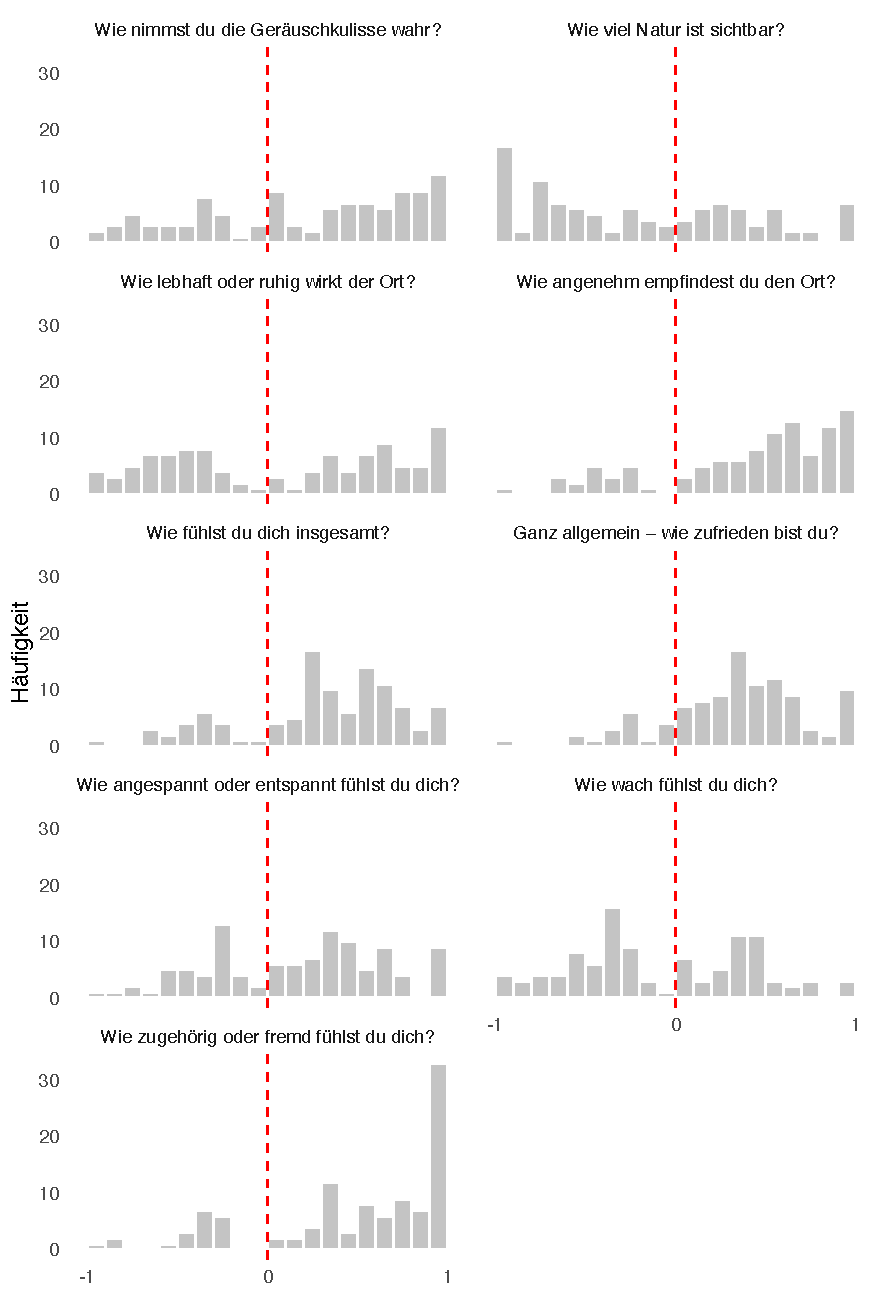
\includegraphics[width=\textwidth]{Analyse/Plots/slider_hists.pdf}
    \caption{Histogramme der Slider-Items}
    \label{fig:slider_hists}
\end{figure}

\begin{longtable}{p{5.5cm}p{9.5cm}}
    \caption{Antworten auf Freitextfragen}
    \label{tab:freitext}\\
    \toprule
    Frage & Antwort \\
    \midrule
    \endfirsthead

    \multicolumn{2}{c}{{\bfseries Tabelle \thetable{} -- Fortsetzung}} \\
    \toprule
    Frage & Antwort \\
    \midrule
    \endhead
    
    \midrule
    \multicolumn{2}{r}{Fortsetzung auf der nächsten Seite}\\
    \endfoot
    
    \bottomrule
    \endlastfoot

    Gibt es andere Dinge die dazu führen, dass Du dich hier weniger wohl oder unwohl fühlst? & heat \\*
     & Everyone is doing the same, so it kind of feels like being at the right place \\*
     & The contact with strangers \\*
     & Bed \\*
     & health issues \\*
     & no natural sunlight room without windows no fresh air \\*
     & a lot of people - personal space \\*
     & No \\*
     & / \\*
     & no \\*
     & Not really \\
    \midrule
    \addlinespace
    Gibt es andere Dinge die dazu führen, dass Du dich hier wohler fühlst? & place i know and is mine i have control over it \\*
     & know this place and can do what i want \\*
     & my room and cozy for the night \\*
     & pets \\*
     & spending time with family pets \\*
     & I am not by myself \\*
     & Less noise from construction works \\
    \bottomrule
\end{longtable}



\addtocontents{toc}{\protect\setcounter{tocdepth}{2}}

\end{appendices}